\begin{figure}[t]			\centering
	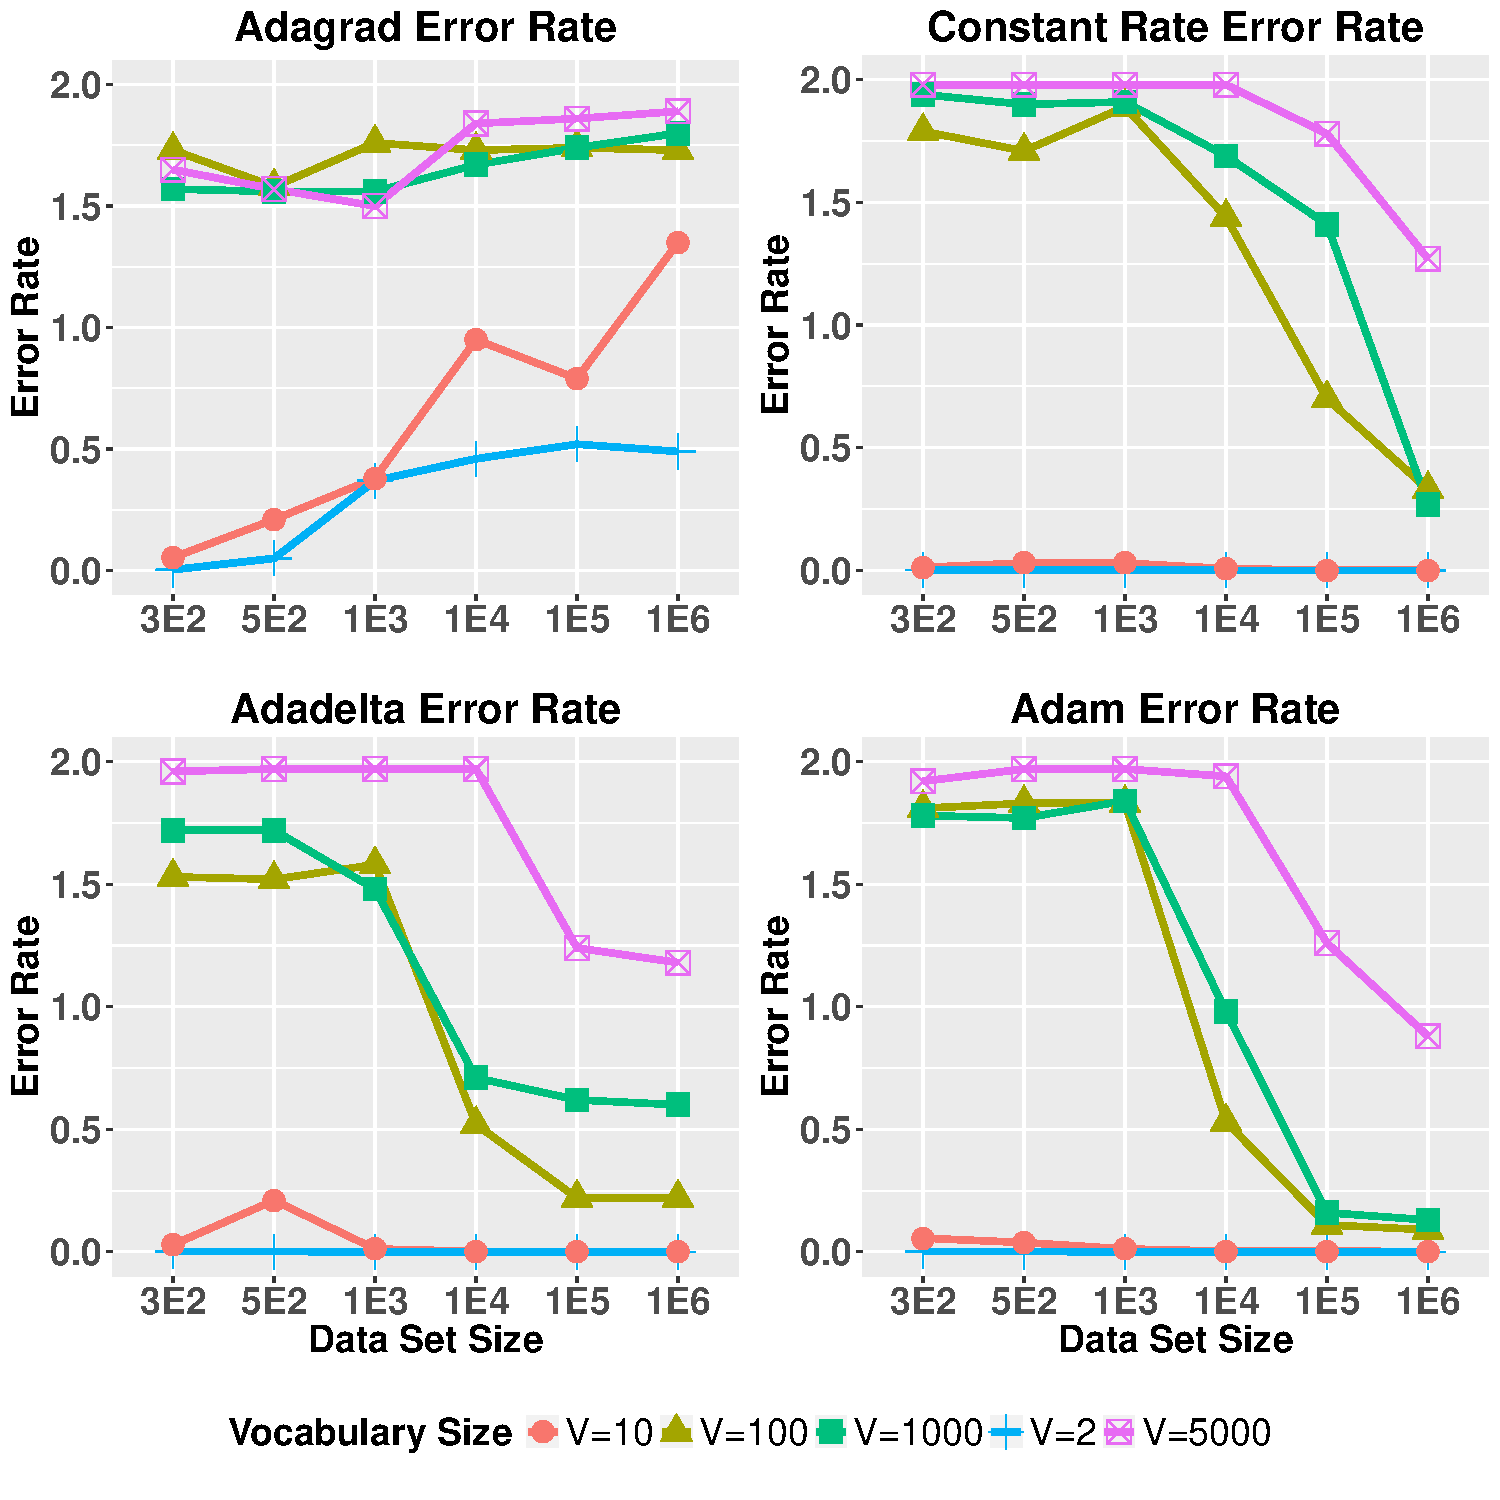
\includegraphics[width= 0.5\textwidth]{2017_emnlp_adagrad_olda/figures/Error-Rate.pdf}

	\caption{Experimental results on synthetic data sets. We vary the vocabulary size $V$, and the number of documents $D$. \abr{adadelta}, \abr{adam} and constant rate perform better with more data, while \abr{adagrad} only does well with small values of $D$.}
	\label{fig:error_rate}       
\end{figure}


\section{Empirical Study}
\label{sec:experiments}



We study three datasets: \textbf{synthetic data}, \textbf{Wikipedia} and
\textbf{\abr{sms} spam
corpus}.\footnote{http://www.esp.uem.es/jmgomez/smsspamcorpus/} We use the
generative process of \abr{lda} to generate synthetic data.
We vary the vocabulary size $V \in \{2, 10, 100,
1000, 5000\}$, and the number of documents $D \in \{300, 500, 10^3, 10^4, 10^5,
10^6\}$.
The \textbf{Wikipedia} dataset consists of 1M articles from
Wikipedia.\footnote{http://www.wikipedia.org}
The vocabulary is the same as~\cite{hoffman2010online}.
The \abr{sms} corpus is a small corpus containing $1084$ documents.




\subsection{Metrics and Settings}





\paragraph{Error rate:} For experiments on synthetic data set, we use
error rate
\begin{equation}
\mbox{Error}(\hat \beta ) = \frac{1}{K} \sum\nolimits_{k = 1}^K {{{\min}_i}||{{\hat \beta }_i} - {\beta _k}|{|_1}}
\end{equation}
to measure the difference between the estimated $\hat{\beta}$ and
the known $\beta$.
The $\min$ greedily matches each $\hat \beta_k$ to its best fit.
While an uncommon metric for unsupervised algorithms,
on the synthetic data we have the true $\beta$.

\paragraph{Predictive likelihood:} For experiments on real data sets, we use
per-word likelihood ~\cite{hoffman2013stochastic} to evaluate the model
quality. We randomly hold out 10K documents and 100 documents on
Wikipedia and \abr{sms} respectively.

\paragraph{Settings:} In the experiments on synthetic data, we use online \abr{lda}~\cite{hoffman2010online}, since the data is generated by \abr{lda}. In the experiments on real datasets, we use online \abr{lda} and online \abr{hdp}~\cite{wang2011online}. In the experiments on Wikipedia, we set the number of topics $K=100$ and
the mini-batch size $M=100$.
In the experiments on \abr{sms} corpus, we set $K=10$ and $M=20$.
For \abr{adam}, we use the default setting of $b$, and set $\rho_0 = 10$ and
$\epsilon = 1000$. For \abr{adadelta}, we set $\epsilon = 1000$. For
\abr{adagrad}, we set $\rho_0 = \epsilon = 1$. These are best settings for
these three methods. The best constant rate is $10^{-3}$.

\subsection{Experimental Results}

\begin{figure}[t]	\centering
			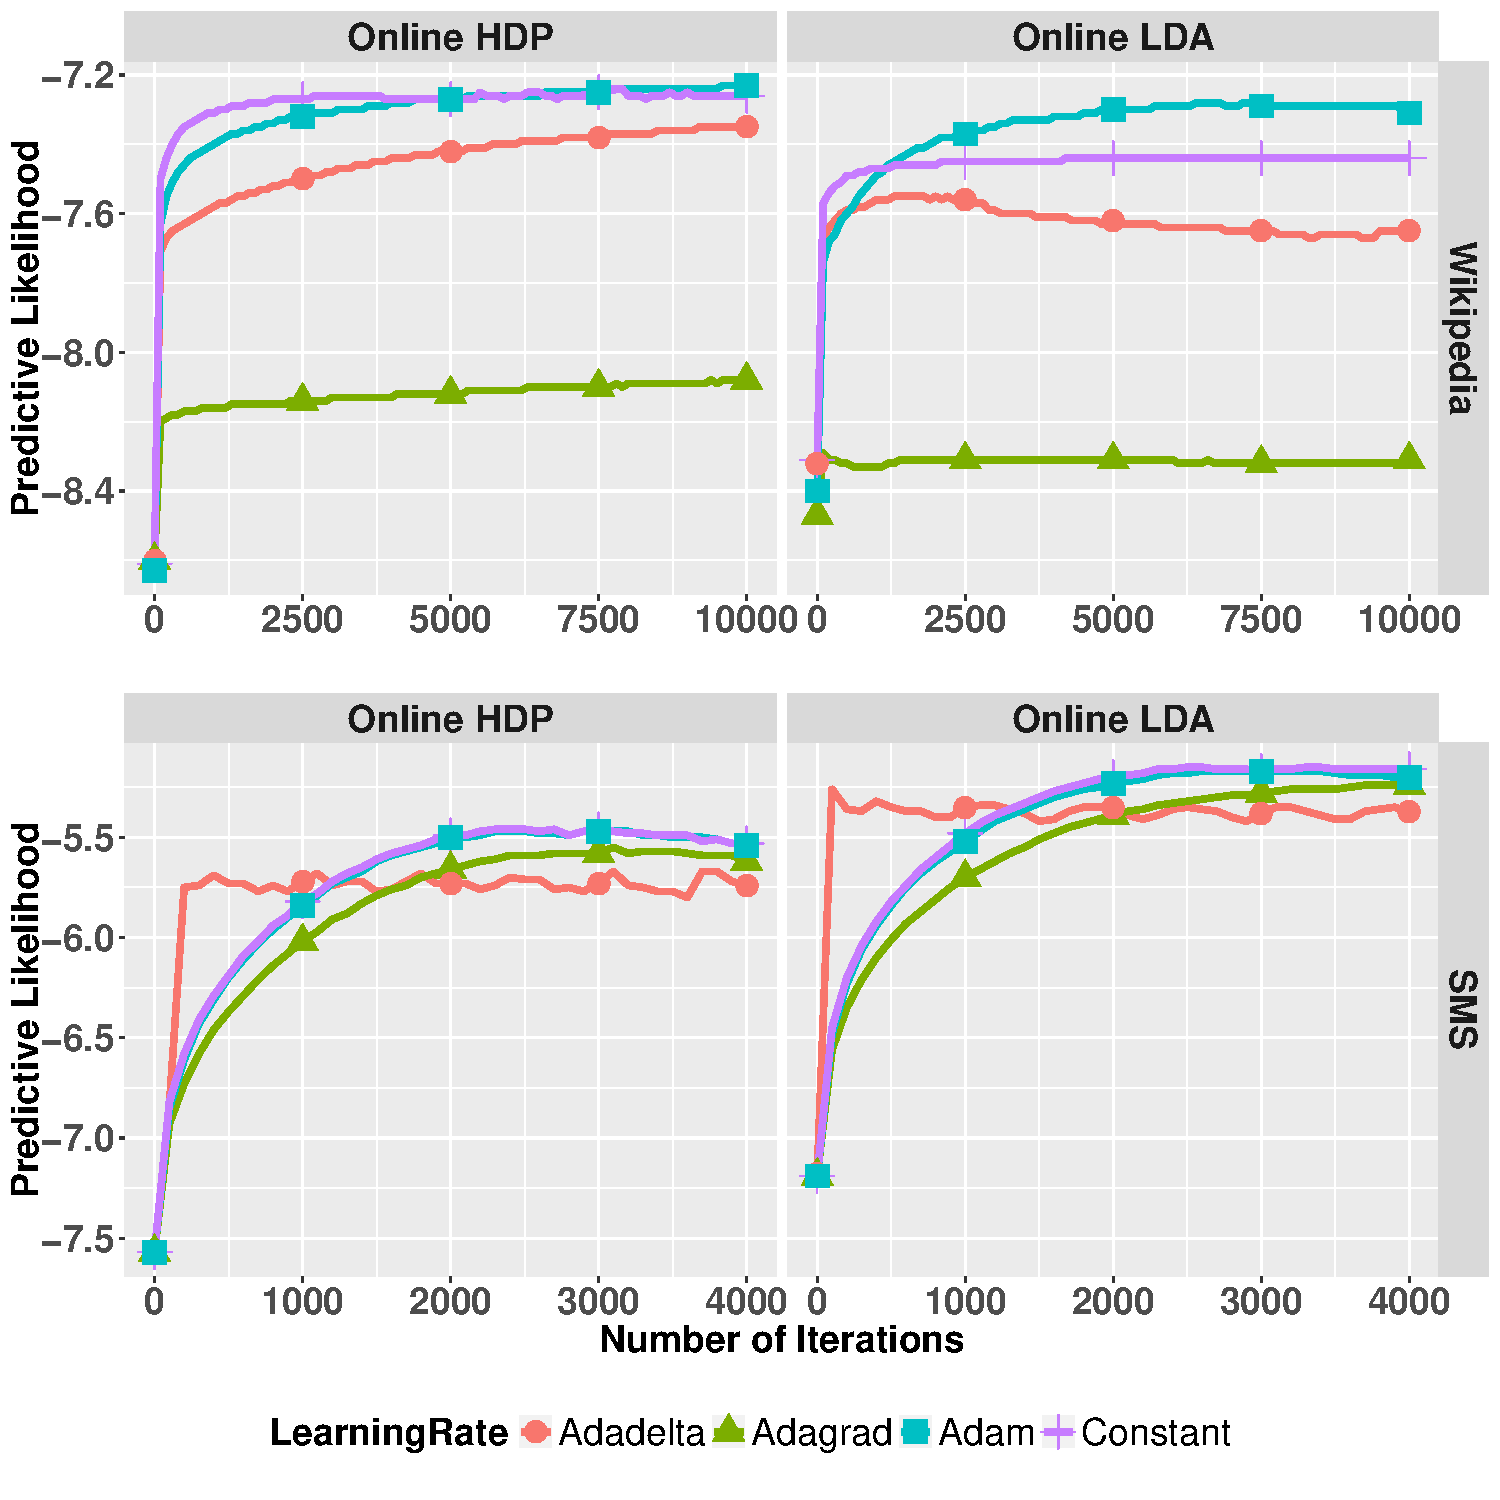
\includegraphics[width= 0.5\textwidth]{2017_emnlp_adagrad_olda/figures/Likelihood.pdf}
		\caption{Experimental results on real corpora. Larger predictive
likelihood is better. On Wikipedia, \abr{adagrad} has does worse than other
methods. On \abr{sms} corpus, \abr{adagrad} is competitive.}
	\label{fig:likelihood}       \end{figure}



Figure~\ref{fig:error_rate} illustrates the experimental results on
synthetic datasets. \abr{adagrad} only works well with small
datasets. When the number of documents increases, \abr{adagrad}
performance degrades. Conversely, other methods can handle more documents.



Figure~\ref{fig:likelihood} illustrates experimental results on real
corpora. \abr{adagrad} gets competitive results to the other
algorithms on the small \abr{sms} corpus. However on very large
Wikipedia corpus, \abr{adagrad} fails to infer good topics, and its
predictive ability is worse than the other methods. While
\abr{adadelta} and \abr{adam} work well on Wikipedia, \abr{adam} is
the clear winner between the two.


